\documentclass[usenames,dvipsnames,aspectratio=169]{beamer}

\usepackage[utf8]{inputenc}
\usepackage[T1]{fontenc}
\usepackage[english]{babel}
\usepackage{indentfirst}
\usepackage{listingsutf8}
\lstset{literate=
  {á}{{\'a}}1 {é}{{\'e}}1 {í}{{\'i}}1 {ó}{{\'o}}1 {ú}{{\'u}}1
  {Á}{{\'A}}1 {É}{{\'E}}1 {Í}{{\'I}}1 {Ó}{{\'O}}1 {Ú}{{\'U}}1
  {à}{{\`a}}1 {è}{{\`e}}1 {ì}{{\`i}}1 {ò}{{\`o}}1 {ù}{{\`u}}1
  {À}{{\`A}}1 {È}{{\'E}}1 {Ì}{{\`I}}1 {Ò}{{\`O}}1 {Ù}{{\`U}}1
  {ä}{{\"a}}1 {ë}{{\"e}}1 {ï}{{\"i}}1 {ö}{{\"o}}1 {ü}{{\"u}}1
  {Ä}{{\"A}}1 {Ë}{{\"E}}1 {Ï}{{\"I}}1 {Ö}{{\"O}}1 {Ü}{{\"U}}1
  {â}{{\^a}}1 {ê}{{\^e}}1 {î}{{\^i}}1 {ô}{{\^o}}1 {û}{{\^u}}1
  {Â}{{\^A}}1 {Ê}{{\^E}}1 {Î}{{\^I}}1 {Ô}{{\^O}}1 {Û}{{\^U}}1
  {œ}{{\oe}}1 {Œ}{{\OE}}1 {æ}{{\ae}}1 {Æ}{{\AE}}1 {ß}{{\ss}}1
  {ç}{{\c c}}1 {Ç}{{\c C}}1 {ø}{{\o}}1 {å}{{\r a}}1 {Å}{{\r A}}1
  {€}{{\EUR}}1 {£}{{\pounds}}1 {ő}{{\H{o}}}1
}
\lstdefinestyle{c}{language=C,
showstringspaces=false,
keywordstyle=\color{MidnightBlue}\bfseries,
stringstyle=\color{DarkOrchid},
commentstyle=\color{Brown},
morecomment=[l][\color{OliveGreen}]{\#}
}
\usepackage{hyperref}
\usepackage{attachfile}
\usepackage{multirow}
\attachfilesetup{color={1.0 0.6 0.0},author={HFM},description={Double click here to show the example},icon=Paperclip}
\usetheme{Warsaw}
\definecolor{kiemelesszin}{rgb}{0.6,0.0,0.0}
\definecolor{hivatkozasszin}{rgb}{0.0,0.0,0.75}
\newcommand{\kiemel}[1]{{\color{kiemelesszin}#1}}
\newcommand{\hiv}[1]{{\color{hivatkozasszin}#1}}
\frenchspacing

\title[Lecture 2.]{Programming basics}
\subtitle{(GKNB\_INTA023)}
\author{Hatwagner F. Miklós, PhD.}
\institute{Széchenyi István University, Győr, Hungary}

\begin{document}

%1
\begin{frame}[plain]
  \titlepage
\end{frame}

%2
\begin{frame}{Square numbers}
  Task: print the squares of the first 10 natural numbers!
  \footnotesize
  \begin{exampleblock}{\textattachfile{squares1.c}{squares1.c}}
      \vspace{-0.3cm}
      \lstinputlisting[style=c]{squares1.c}    
      \vspace{-0.3cm}
  \end{exampleblock}
\end{frame}

%3
\begin{frame}[fragile]{Square numbers}
  \footnotesize
  \begin{block}{Output}
    \begin{verbatim}
Squares of natural numbers

1^2=1
2^2=4
3^2=9
4^2=16
5^2=25
6^2=36
7^2=49
8^2=64
9^2=81
10^2=100
\end{verbatim}
  \end{block}
  Problems:
  \begin{itemize}
    \item \kiemel{We have calculated the results, not the computer!}
    \item Too much repeating, similar lines of code
    \item Very easy to make mistakes, but hard to realize them
  \end{itemize}
\end{frame}

%4
\begin{frame}{Square numbers}
  Task: do the computer calculate the square numbers!
  \footnotesize
  \begin{exampleblock}{\textattachfile{squares2.c}{squares2.c}}
      \lstinputlisting[style=c,linerange={1-9},numbers=left,firstnumber=1]{squares2.c}
      \lstinputlisting[style=c,linerange={13-15},numbers=left,firstnumber=14]{squares2.c}
  \end{exampleblock}
\end{frame}

%5
\begin{frame}[fragile]{Square numbers}
  \begin{columns}[c]
    \column{0.5\textwidth}
      \scriptsize
      \begin{block}{Output}
        \begin{verbatim}
Squares of natural numbers

1^2=1
2^2=4
3^2=9
4^2=16
5^2=25
6^2=36
7^2=49
8^2=64
9^2=81
10^2=100
\end{verbatim}
      \end{block}  
    \column{0.5\textwidth}
      Literals: constant values typed in the source code
    \begin{itemize}
      \item Integer constants
      \item Character constants: between \kiemel{'}-s
      \item String constants: between \kiemel{"}-s
    \end{itemize}
  \end{columns}
  \begin{center}
    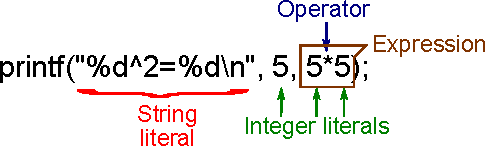
\includegraphics[]{printf1.pdf}
  \end{center}
\end{frame}

%6
\begin{frame}{Square numbers}
  Expression: produces a value by using literals (constants), variables and operators
  \begin{center}
    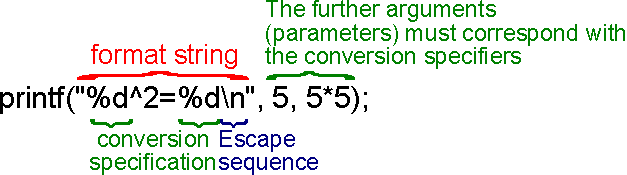
\includegraphics[scale=.9]{printf2.pdf}
  \end{center}
  Some arithmetic operators\\
  \begin{center}
    \begin{tabular}{lll}
      Operator & Description & Example\\ \hline
      \texttt{+} & Addition & $5 + 3 == 8$ \\
      \texttt{-} & Subtraction & $5 - 3 == 2$ \\
      \texttt{*} & Multiplication & $5 * 3 == 15$ \\
      \texttt{/} & Integer division ($\to$ quotient) & $5 / 3 == 1$ \\
      \texttt{\%} & Modulo ($\to$ remainder) & $5 \% 3 == 2$ \\
    \end{tabular}
  \end{center}
\end{frame}

%7
\begin{frame}{Square numbers}
  \footnotesize
  \begin{exampleblock}{\textattachfile{squares3.c}{squares3.c}}
    \vspace{-0.3cm}
    \lstinputlisting[style=c,linerange={1-11},numbers=left,firstnumber=1]{squares3.c}
    \lstinputlisting[style=c,firstline=24,numbers=left,firstnumber=24]{squares3.c}
    \vspace{-0.3cm}
  \end{exampleblock}
\end{frame}

%8
\begin{frame}{Square numbers}
  Variables
  \begin{itemize}
    \item Eg. \texttt{int base;}
    \item type
    \begin{itemize}
      \item the nature of data (numeric, text)
      \item data representation
      \item possible operations
    \end{itemize}
    \item memory area
    \begin{itemize}
      \item stores the value according to the type
      \item the initial value of local variables (in blocks between \kiemel{\{} and \kiemel{\}}) is undefined, ``garbage''
    \end{itemize}
    \item name, id (should refer to its goal)
  \end{itemize}
\end{frame}

%9
\begin{frame}{Square numbers}
  Naming rules
  \begin{itemize}
    \item Fist character: lower-, uppercase letter or \_
    \item Further characters: the same set of characters and digits as well
    \item Cannot be a reserved keyword or identifier
    \item Case sensitive
    \item Recommendation: do not start the names with one or two \_ characters
    \item Number of significant characters
  \end{itemize}
  \begin{columns}[T]
    \column{.5\textwidth}
      \begin{alertblock}{What's the problem?}
        John Doe\\
        12\_Monkeys\\
        Cool!\\
        auto
      \end{alertblock}
    \column{.5\textwidth}
      \begin{exampleblock}{OK}
        john\_doe\\
        John\_Doe\\
        johnDoe
      \end{exampleblock}
  \end{columns}
\end{frame}

%10
\begin{frame}{Square numbers}
  The most important integer types (fixed point arithmetic)
  \scriptsize
  \begin{center}
    \begin{tabular}{ll}
      Type & Description \\ \hline\hline
      \texttt{char} & Generally signed, 8 bit integer \\ \hline
      \texttt{signed char} & Signed 8 bit integer \\ \hline
      \texttt{unsigned char} & Unsigned (non negative) 8 bit integer \\ \hline
      \texttt{short} & \multirow{3}{*}{Signed short integer} \\
      \texttt{signed short} & \\
      \texttt{signed short int} & \\ \hline
      \texttt{unsigned short} & \multirow{2}{*}{Unsigned short integer} \\
      \texttt{unsigned short int} & \\ \hline
      \texttt{signed} & \multirow{3}{*}{Signed integer} \\
      \texttt{int} & \\
      \texttt{signed int} & \\ \hline
      \texttt{unsigned} & \multirow{2}{*}{Unsigned integer} \\
      \texttt{unsigned int} & \\ \hline
      \texttt{long} & \multirow{3}{*}{Signed long integer} \\
      \texttt{signed long} & \\
      \texttt{signed long int} & \\ \hline
      \texttt{unsigned long} & \multirow{2}{*}{Unsigned long integer} \\
      \texttt{unsigned long int} & \\
    \end{tabular}
  \end{center}
\end{frame}

%11
\begin{frame}{Square numbers}
  Remarks:
  \begin{itemize}
    \item (Type) modifiers: \texttt{signed/unsigned}, \texttt{short/long}
    \item Storage of integer literals: \texttt{int}
    \item Size of type \texttt{char} is always 1 byte, but character literals are stored as \texttt{int}!
    \item Sign of \texttt{char} depends on the platform / compiler, but it is usually signed (can be modified)
    \item \texttt{1 == sizeof(char) <= sizeof(short) <= sizeof(int) <= sizeof(long) <= sizeof(long long)}, where \texttt{sizeof} 
is an operator that specifies the size of a type / variable in bytes
  \end{itemize}
\end{frame}

%12
\begin{frame}{Square numbers}
  Variable definition
  \begin{itemize}
    \item General usage: \emph{type variable\_list;}
    \item Defines a name, type and allocates memory to store the data
    \item Eg. \kiemel{\texttt{int x; int i, j, k; unsigned int y;}}
  \end{itemize}
  Assignment
  \begin{itemize}
    \item Operator: \kiemel{=}
    \item \emph{lvalue} \kiemel{=} \emph{rvalue};
    \item changes the value of \emph{lvalue} to \emph{rvalue}
    \item \emph{lvalue}: generally a variable (it cannot be a literal or an array, but a specific element of an array is allowed)
  \end{itemize}
  \vfill
  Result: the rows of our program are very similar, can be copied\\
  Problem: many repeating code parts $\to$ let the computer repeat the same parts!
\end{frame}

%13
\begin{frame}{Square numbers}
  \footnotesize
  \begin{exampleblock}{\textattachfile{squares4.c}{squares4.c}}
      \lstinputlisting[style=c]{squares4.c}    
  \end{exampleblock}
\end{frame}

%14
\begin{frame}{Square numbers}
  Relational operators
  \begin{center}
    \begin{tabular}{ll}
      Operator & Description \\ \hline
      \texttt{==} & Equal to \\
      \texttt{!=} & Not equal to \\
      \texttt{<} & Less than \\
      \texttt{<=} & Less than or equal to \\
      \texttt{>} & Greater than \\
      \texttt{>=} & Greater than or equal to \\
    \end{tabular}
  \end{center}
\end{frame}

%15
\begin{frame}{Square numbers}
  while loop (tests the condition \emph{before} executing the loop body)
  \vfill
  \emph{while(condition) \{} \\
  \hspace{0.5cm} \emph{activities}\\
  \emph{\}}\\
  \vfill
  The \emph{body} (repeated part) of the loop may contain
  \begin{itemize}
    \item a single statement
    \item a group of statements (block between \kiemel{\{} and \kiemel{\}})
  \end{itemize}
\end{frame}

%16
\begin{frame}{Flow charts}
  \begin{columns}[T]
    \column{0.25\textwidth}
      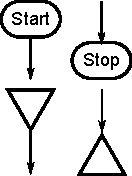
\includegraphics{./startend.pdf}
    \column{0.75\textwidth}
      Signals of start and end
      \begin{itemize}
        \item Triangle version: description of algorithm parts
        \item A program must contain exactly one start and one end point
        \item The start point must have a sole outgoing arrow only. The end point\dots
      \end{itemize}
  \end{columns}
  \vfill
  \begin{columns}[T]
    \column{0.25\textwidth}
      
\includegraphics{./direction.pdf}
    \column{0.75\textwidth}
      Signal of direction
      \begin{itemize}
        \item May diverge only at conditions
        \item Shows the execution order of instructions
      \end{itemize}
  \end{columns}
\end{frame}

%17
\begin{frame}{Flow charts}
  \begin{columns}[T]
    \column{0.35\textwidth}
      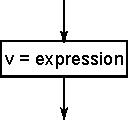
\includegraphics{./assignment.pdf}
    \column{0.65\textwidth}
      Signal of assignment
      \begin{itemize}
        \item One arrow comes in, one goes out
        \item The value and type of the \emph{expression} must be defined, then this value is going to be assigned to variable \emph{v}
        \item Multiple assignments can be grouped together
      \end{itemize}
  \end{columns}
  \vfill
  \begin{columns}[T]
    \column{0.35\textwidth}
      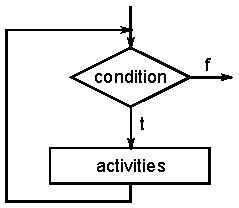
\includegraphics{testBefore.pdf}
    \column{0.65\textwidth}
      Loop (tests the condition before executing the loop body)
      \begin{itemize}
        \item Loop body: the repeated activities
        \item The loop body must affect the condition $\to$ infinite loop?
        \item The loop body may never be executed
      \end{itemize}
  \end{columns}
\end{frame}

%18
\begin{frame}{Flow charts}
  \begin{columns}[T]
    \column{0.25\textwidth}
      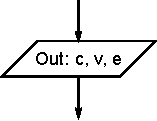
\includegraphics{./output.pdf}
    \column{0.75\textwidth}
      Signal of output activity (print)
      \begin{itemize}
        \item One arrow comes in, one goes out
        \item The values of the \emph{c} constant, \emph{v} variable and \emph{e}
expression must be printed
      \end{itemize}
  \end{columns}
\end{frame}

%19
\begin{frame}{Square numbers}
  \begin{center}
    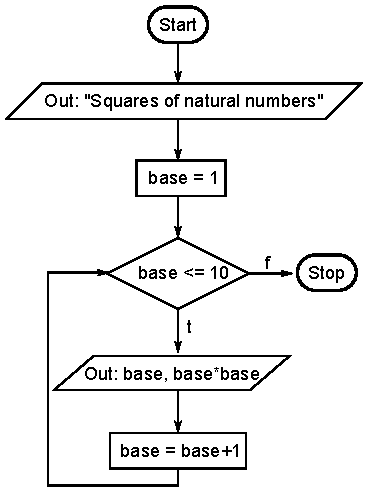
\includegraphics[scale=0.8]{./squares4.pdf}
  \end{center}
\end{frame}

%20
\begin{frame}{Square numbers}
  Table of data structure: the flow chart defines neither the type nor the goal of variables
  \vfill
  \begin{center}
    \begin{tabular}{llll}
    Goal & Name & Type & Nature\\ \hline
    Base of power & base & integer & work/output \\
    \end{tabular}
  \end{center}
\end{frame}

%21
\begin{frame}{Even, odd}
  Make a decision: is a specific number odd or even?
  \begin{exampleblock}{\textattachfile{even1.c}{even1.c}}
    \footnotesize
    \lstinputlisting[style=c]{even1.c}
  \end{exampleblock}
\end{frame}

%22
\begin{frame}{Even, odd}
  Conditions
  \vfill
  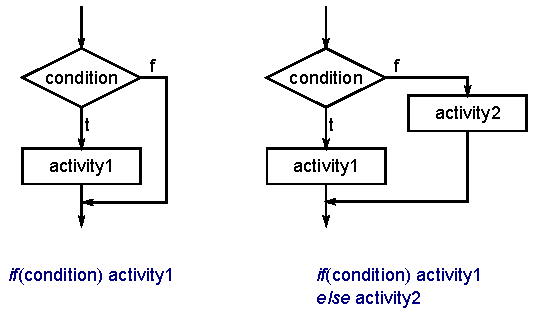
\includegraphics[width=.7\textwidth]{condition.pdf}
  \vfill
  Nested if-else statements are possible for multiple outcomes
\end{frame}

%23
\begin{frame}[fragile]{Pointers}
  What is a \emph{pointer}, and what is it good for?
  \begin{itemize}
    \item A type suitable to store a memory address
    \item Several subtypes exist to express the type of the stored data
    \item In the technical sense, they are non-negative integer numbers
    \item Pointer definition: \emph{base\_type}* \emph{name};
  \end{itemize}
  \begin{exampleblock}{Example}
    \small
    \begin{verbatim}
int i;          // integer variable

int* pi;        // pointer variable that stores 
                // the address of an integer variable
\end{verbatim}
  \end{exampleblock}
\end{frame}

%24
\begin{frame}{Pointers}
  The \emph{address} of a variable can be obtained by operator \kiemel{\&}\\
  The \emph{content} of a variable \emph{at a specific address} can be obtained by operator \kiemel{*} (indirection, dereference)\\
  \begin{exampleblock}{\textattachfile{pointer.c}{pointer.c}}
    \vspace{-.3cm}
    \footnotesize
    \lstinputlisting[style=c]{pointer.c}
    \vspace{-.3cm}
  \end{exampleblock}
\end{frame}

%25
\begin{frame}[fragile]{Pointers}
  \begin{block}{Output}
    \begin{verbatim}
The value of 'i' is: 42
The address of 'i' is: 0x7ffe2c9fe634
The value at address 'pi' is: 42
The value of 'pi' is: 0x7ffe2c9fe634
The address of 'pi' is: 0x7ffe2c9fe638
\end{verbatim}
  \end{block}
  The format specifier of a pointer is: \kiemel{\%p}\\
  \begin{exampleblock}{}
    \footnotesize
    \lstinputlisting[style=c,linerange={7-7}]{pointer.c}
  \end{exampleblock}
\end{frame}

%26
\begin{frame}{Pointers}
  \begin{center}
    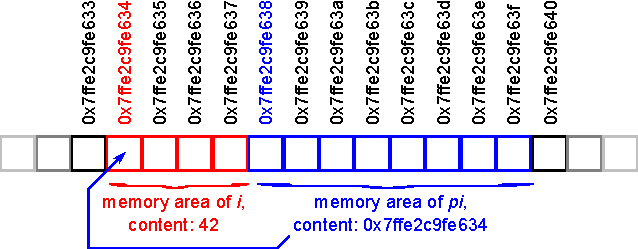
\includegraphics[scale=1.25]{pointer.pdf}
  \end{center}
\end{frame}

%27
\begin{frame}{Even, odd}
  Task: let the program read the number to analize!
  \begin{exampleblock}{\textattachfile{even2.c}{even2.c}}
    \footnotesize
    \lstinputlisting[style=c]{even2.c}
  \end{exampleblock}
\end{frame}

%28
\begin{frame}{Even, odd}
  \begin{exampleblock}{}
    \footnotesize
    \lstinputlisting[style=c,linerange={5-6}]{even2.c}
  \end{exampleblock}
  The preprocessor merges the string literals if they are separated by only a \emph{whitespace} character.
  \begin{exampleblock}{}
    \footnotesize
    \lstinputlisting[style=c,linerange={7-7}]{even2.c}
  \end{exampleblock}
  Reading from the standard input
  \begin{itemize}
    \item \texttt{\kiemel{scanf}} is the ``inverse'' of printf
    \item Its first argument is the format string (similarly to \texttt{printf})
    \item The following arguments must match the applied format specifiers
    \item The \emph{address} of variables that store the read, converted values must be given
  \end{itemize}
\end{frame}

%29
\begin{frame}{Even, odd}
  \begin{center}
    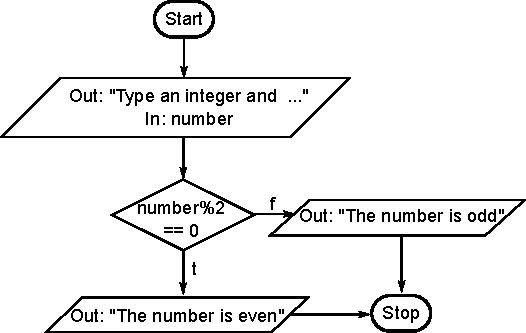
\includegraphics[]{even2.pdf}
  \end{center}
\end{frame}

%30
\begin{frame}{Even, odd}
  Order of instructions (expressions)
  \begin{itemize}
    \item parenthesis
    \item precedence
  \end{itemize}
  \begin{center}
    \begin{tabular}{ll}
    Operator & Associativity\\ \hline
    sizeof & right to left\\
    * / \% & left to right\\
    + - & left to right\\
    < <= > >= & left to right\\
    == != & left to right\\
    = & right to left\\
    \end{tabular}
  \end{center}
  Control structures
  \begin{itemize}
    \item Sequence (Statements are executed in a specified order. No statement is skipped and no statement is executed more than once.)
    \item Repetition (loop, iteration)
    \item Selection (condition)
  \end{itemize}
\end{frame}

\end{document}
